\documentclass[10pt]{beamer}
\usetheme{metropolis}
\usepackage{booktabs}
\usepackage{tabularx}
\usepackage{calc}
\usepackage{tikz}

% Setup for faculty images
\newlength{\imageheight}
\setlength{\imageheight}{3.5cm}

% Define CSUF brand colors
\definecolor{titanblue}{HTML}{00244E}
\definecolor{mediumblue}{HTML}{0F3F8C}
\definecolor{skyblue}{HTML}{EBFBFF}
\definecolor{titanorange}{HTML}{FF7900}
\definecolor{titangray}{HTML}{F5F5F5}
\definecolor{titantext}{HTML}{222222}

% Customize metropolis theme colors
\setbeamercolor{normal text}{fg=titantext, bg=white}
\setbeamercolor{alerted text}{fg=titanorange}
\setbeamercolor{example text}{fg=mediumblue}

% Title page colors
\setbeamercolor{title}{fg=titanblue, bg=white}
\setbeamercolor{subtitle}{fg=mediumblue, bg=white}
\setbeamercolor{institute}{fg=titanorange, bg=white}
\setbeamercolor{date}{fg=titanblue, bg=white}

% Frame title colors
\setbeamercolor{frametitle}{fg=white, bg=titanblue}
\setbeamercolor{framesubtitle}{fg=mediumblue, bg=white}


% Block environment colors
\setbeamercolor{block title}{fg=white, bg=titanblue}
\setbeamercolor{block body}{fg=titantext, bg=skyblue!10}

% Item colors
\setbeamercolor{itemize item}{fg=titanorange}
\setbeamercolor{itemize subitem}{fg=mediumblue}
\setbeamercolor{itemize subsubitem}{fg=titanblue}

% Footer and header colors
\setbeamercolor{footer}{fg=titantext}
\setbeamercolor{header}{fg=titanblue}

% Customize fonts
\setbeamerfont{title}{size=\Large, series=\bfseries}
\setbeamerfont{frametitle}{size=\large, series=\bfseries}

% Simple title page template
\defbeamertemplate*{title page}{customized}[1][]
{
    \vspace{1cm}
    {\usebeamerfont{title}\usebeamercolor[fg]{title}\inserttitle\par}
    \vspace{0.5cm}
    {\usebeamerfont{subtitle}\usebeamercolor[fg]{subtitle}\insertsubtitle\par}
    \vspace{0.5cm}
    {\usebeamerfont{date}\usebeamercolor[fg]{date}\insertdate\par}
    \vfill
    {\insertinstitute\par}
}

% Add progress bar
\makeatletter
\setbeamertemplate{headline}{%
  \begin{beamercolorbox}[wd=\paperwidth,ht=0.4cm,dp=0cm]{titanblue}%
    \begin{tikzpicture}
      \fill[titanorange] (0,0) rectangle (\the\paperwidth*\insertframenumber/\inserttotalframenumber,0.4cm);
    \end{tikzpicture}%
  \end{beamercolorbox}%
}
\makeatother
\begin{document}

\title{Master of Public Administration Program}
\subtitle{MPA Student Orientation}
\date{Spring 2025}
\institute{
\includegraphics[width=.8\textwidth]{images/PUBLIC-ADMINISTRATION-color2.png}}

\maketitle


\begin{frame}{Agenda}
\begin{itemize}
\item Welcome and Program Overview
\item Introductions
\item Program Structure and Requirements
\item Faculty Profiles
\item Academic Information
\item Program Resources and Scholarships
\item Campus Resources
\item Questions \& Answers
\end{itemize}
\end{frame}

\begin{frame}{Program by the Numbers}
\begin{itemize}
\item Awarding degrees since 1968
\item The only public MPA in Orange County
\item 83 Students in the Program
\item $\sim$30 Graduates each Year
\item Four Concentrations
\item Three years typical to complete the program
\end{itemize}
\end{frame}

\begin{frame}{The Value of a CSUF MPA}
\begin{itemize}
\item \#1: Most selective public MPA program in Southern California
\item 13.3: Lowest student-to-faculty ratio of any public MPA program in Southern California
\item 1,100+: Alumni network serving in all levels of government and nonprofit/private sectors
\item Continuously accredited by NASPAA since the 1980s
\end{itemize}
\end{frame}

\begin{frame}{Our Mission}
    \textbf{Mission}\\
    We prepare leaders to address complex social issues, uphold democratic values, and foster a commitment to ethical, equitable, and inclusive public service in Orange County and beyond.
    
    \vspace{1em}
    
    \textbf{Vision}\\
    Our vision is to be a program recognized for excellence in value-driven public service and community engagement.
    
    \vspace{1em}
    
    \textbf{Values}
    \begin{itemize}
    \item Accountability
    \item Ethics
    \item Collaboration
    \item Life-long Learning
    \end{itemize}
\end{frame}

\begin{frame}{MPA Program Faculty}
    \begin{columns}[T]
    \column{0.65\textwidth}
    \textbf{Core Faculty Members}
    \begin{itemize}
    \item Nine full-time faculty members
    \item Diverse research interests and expertise
    \item Strong professional experience
    \item Active in research and community engagement
    \end{itemize}
    \column{0.35\textwidth}
    \includegraphics[height=\imageheight]{images/gordon_hall.jpg}
    \end{columns}
    \end{frame}
    
    \begin{frame}{Program Director}
    \begin{columns}[T]
    \column{0.65\textwidth}
    \textbf{David P. Adams, Ph.D.}
    \begin{itemize}
    \item Associate Professor and MPA Director
    \item At CSUF since 2016
    \item Ph.D. from Auburn University
    \end{itemize}
    
    \textbf{Research:}
    \begin{itemize}
    \item Public Policy Outcomes
    \item Collaboration
    \item Environmental and Energy Policy
    \item Environmental Justice
    \end{itemize}
    
    \textbf{Courses:} Foundations of PA, Capstone Seminar, Collaborative Governance
    
    \column{0.35\textwidth}
    \vspace*{0.5cm} % Adjust vertical spacing
    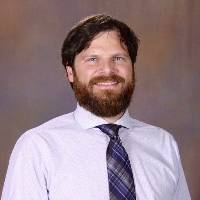
\includegraphics[height=\imageheight]{images/adams.jpg}
    \end{columns}
    \end{frame}
        
    \begin{frame}{Faculty Profile}
    \begin{columns}[T]
    \column{0.65\textwidth}
    \textbf{Shelly Arsneault, Ph.D.}
    \begin{itemize}
    \item Professor and Vice Chair of PAJ
    \item At CSUF since 2002
    \item Ph.D. from Michigan State University
    \item Editorial Board, Journal of Public Affairs Education
    \end{itemize}
    
    \textbf{Research:} 
    \begin{itemize}
    \item Nonprofit Management
    \item Education Policy
    \end{itemize}

    \textbf{Courses:} Foundations of PA, Nonprofit Management, Education Policy
    
    \column{0.35\textwidth}
    \vspace*{0.5cm}
    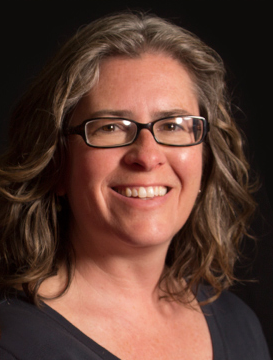
\includegraphics[height=\imageheight]{images/arsneault.png}
    \end{columns}
    \end{frame}

    \begin{frame}{Faculty Profile}
        \begin{columns}[T]
        \column{0.65\textwidth}
        \textbf{Sean Angst, Ph.D.}
        \begin{itemize}
        \item Ph.D. from USC Price School
        \item At CSUF since 2024
        \end{itemize}
        
        \textbf{Research Focus:}
        \begin{itemize}
        \item Housing Policy
        \item Community Development
        \item Racial Justice
        \end{itemize}
        
        \textbf{Courses:} 
        \begin{itemize}
        \item Administrative Research and Analysis
        \item Policy Analysis
        \end{itemize}
        \column{0.35\textwidth}
        \vspace*{0.5cm}
        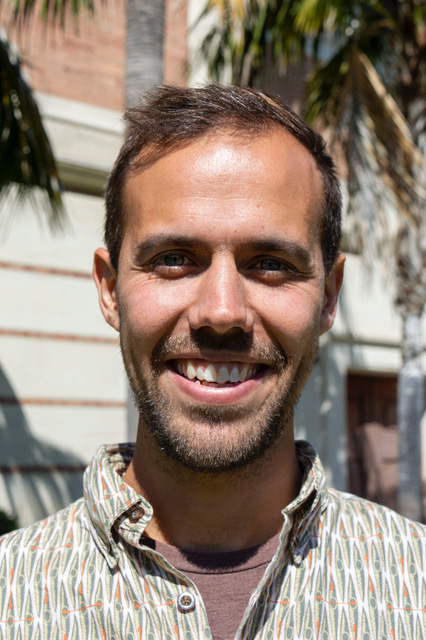
\includegraphics[height=\imageheight]{images/angst.jpg}
        \end{columns}
        \end{frame}
        
        \begin{frame}{Faculty Profile}
        \begin{columns}[T]
        \column{0.65\textwidth}
        \textbf{Meriem Doucette, Ph.D.}
        \begin{itemize}
        \item Associate Professor
        \item At CSUF since 2015
        \item Ph.D. from University of Georgia
        \end{itemize}
        
        \textbf{Research:} 
        \begin{itemize}
        \item Organizational Theory
        \item Change Management
        \end{itemize}

        \textbf{Courses:} 
        \begin{itemize}
        \item Organizational Theory
        \item Ethics
        \item Organizational Development
        \item Leadership
        \end{itemize}
        \column{0.35\textwidth}
        \vspace*{0.5cm}
        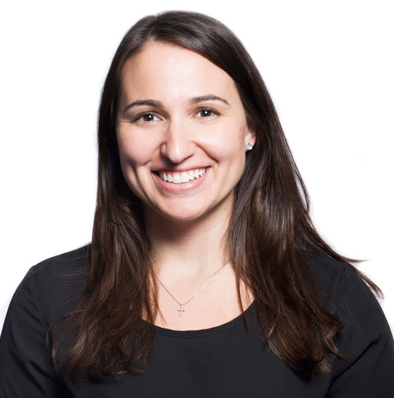
\includegraphics[height=\imageheight]{images/doucette.png}
        \end{columns}
        \end{frame}
        
        \begin{frame}{Faculty Profile}
        \begin{columns}[T]
        \column{0.65\textwidth}
        \textbf{Elaine Frey, Ph.D.}
        \begin{itemize}
        \item Ph.D. from George Washington University
        \end{itemize}
        
        \textbf{Research Areas:}
        \begin{itemize}
        \item Environmental Economics
        \item Energy Economics
        \item Applied Microeconomics
        \end{itemize}
        
        \textbf{Courses:} 
        \begin{itemize}
        \item Environmental Policy
        \item Administrative Research and Analysis
        \end{itemize}
        
        \column{0.35\textwidth}
        \vspace*{0.5cm}
        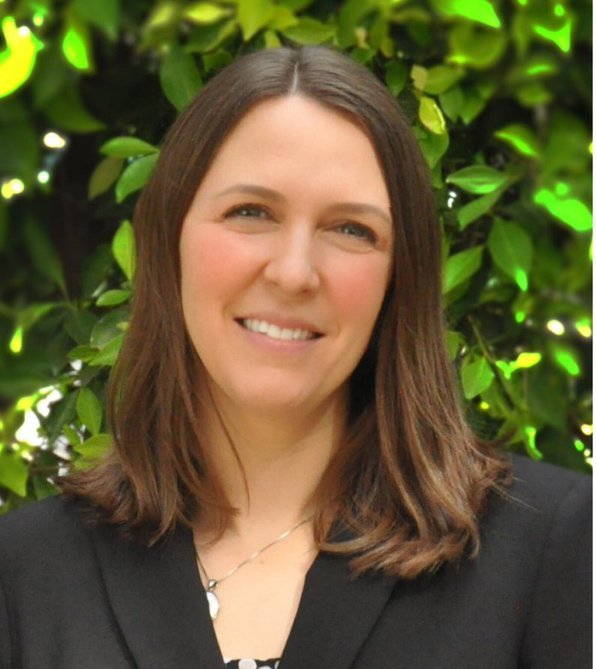
\includegraphics[height=\imageheight]{images/frey.jpg}
        \end{columns}
        \end{frame}
        
        \begin{frame}{Faculty Profile}
        \begin{columns}[T]
        \column{0.65\textwidth}
        \textbf{Sarah A. Hill, Ph.D.}
        \begin{itemize}
        \item Professor
        \item At CSUF since 2007
        \item Ph.D. from California Institute of Technology
        \end{itemize}
        
        \textbf{Research:} 
        \begin{itemize}
            \item Elections Administration
            \item Education Policy
        \end{itemize}

        \textbf{Courses:} 
        \begin{itemize}
        \item State \& Local Government
        \item Public Policy
        \item Diversity in Public Management
        \end{itemize}
        \column{0.35\textwidth}
        \vspace*{0.5cm}
        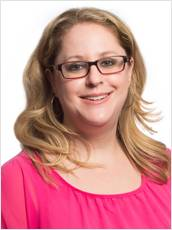
\includegraphics[height=\imageheight]{images/hill.jpg}
        \end{columns}
        \end{frame}
        
        \begin{frame}{Faculty Profile}
        \begin{columns}[T]
        \column{0.65\textwidth}
        \textbf{Myung-Jung "MJ" Kwon, Ph.D.}
        \begin{itemize}
        \item Professor and MPA Advisor
        \item At CSUF since 2009
        \item Ph.D. from Florida State University
        \item Editorial Board, International Journal of Public Administration
        \end{itemize}
        
        \textbf{Research:}
        \begin{itemize}
        \item Public Sector Innovation
        \item E-Government
        \end{itemize}
        
        \textbf{Courses:}
        \begin{itemize}
        \item Human Resources Management
        \item Public Personnel Administration
        \item Diversity in Public Management
        \end{itemize}

        \column{0.35\textwidth}
        \vspace*{0.5cm}
        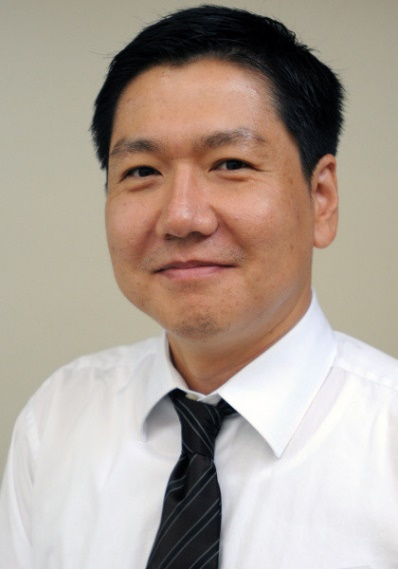
\includegraphics[height=\imageheight]{images/kwon.jpg}
        \end{columns}
        \end{frame}
    
        \begin{frame}{Faculty Profile}
        \begin{columns}[T]
        \column{0.65\textwidth}
        \textbf{Samuel B. Stone, Ph.D.}
        \begin{itemize}
        \item Professor
        \item At CSUF since 2011
        \item Ph.D. from Indiana University
        \end{itemize}
        
        \textbf{Research:}
        \begin{itemize}
        \item Financial Analysis
        \item Fiscal Policy
        \item Local Government Management
        \end{itemize}
        
        \textbf{Courses:}
        \begin{itemize}
        \item Public Finance
        \item Public Budgeting
        \item Local Government Management
        \end{itemize}

        \column{0.35\textwidth}
        \vspace*{0.5cm}
        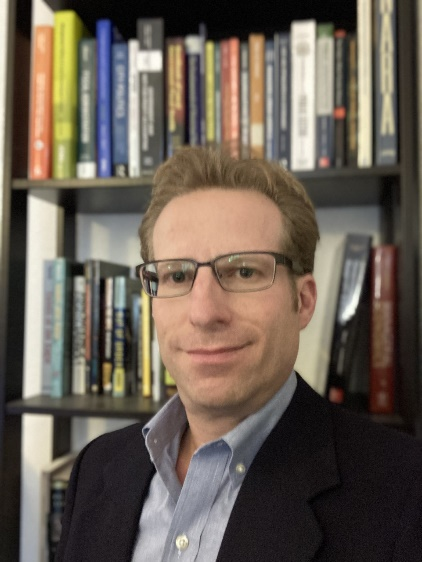
\includegraphics[height=\imageheight]{images/stone.jpg}
        \end{columns}
        \end{frame}

\begin{frame}{Faculty Profile}
\begin{columns}[T]
\column{0.65\textwidth}
\textbf{Yuan Ting, Ph.D.}
\begin{itemize}
\item Professor
\item At CSUF since 1991
\item Ph.D. from Northern Illinois University
\end{itemize}

\textbf{Research:}
\begin{itemize}
\item Performance Measurement
\item Job Satisfaction
\item Public Sector Management
\end{itemize}

\textbf{Courses:}
\begin{itemize}
\item Human Resources Management
\item Public Personnel Admin.
\item Capstone Seminar
\end{itemize}
\column{0.35\textwidth}
\vspace*{0.5cm}
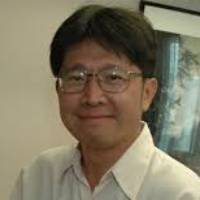
\includegraphics[height=\imageheight]{images/ting.jpg}
\end{columns}
\end{frame}

\begin{frame}{Affiliated Faculty Profile}
    \begin{columns}[T]
    \column{0.65\textwidth}
    \textbf{Scott Spitzer, Ph.D.}
    \begin{itemize}
    \item Professor
    \item At CSUF since 2006
    \item Ph.D. from Columbia University
    \end{itemize}
    
    \textbf{Research:} 
    \begin{itemize}
    \item Urban Politics
    \item Racial Politics
    \item Social Welfare
    \end{itemize}

    \textbf{Courses:} 
    \begin{itemize}
    \item Urban Politics
    \item Metropolitan Politics and Policy
    \end{itemize}
    
    \column{0.35\textwidth}
    \vspace*{0.5cm}
    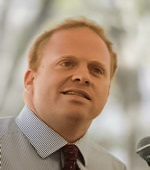
\includegraphics[height=\imageheight]{images/spitzer.png}
    \end{columns}
    \end{frame}
    
\begin{frame}{Academic Information}
\begin{itemize}
\item Program Structure
\item Concentrations
\item Program Milestones
\item Scholarships \& Awards
\item Graduation Awards
\item Keys to Graduate School Success
\item Campus Resources Overview
\end{itemize}
\end{frame}


\begin{frame}{Program Structure}
\begin{itemize}
\item Total Units: 36 (12 courses)
\item Prerequisites
\item Core courses
\item Concentration
\item Electives
\item Internship (required for students without public sector experience)
\item Comprehensive Exam
\end{itemize}
\end{frame}

\begin{frame}{Concentrations}
Choose one concentration:
\begin{itemize}
\item Human Resource Management
\item Local Government Management
\item Public Finance
\item Public Policy
\end{itemize}
Concentrations should be complementary, not supplementary
\end{frame}


\begin{frame}{Program Milestones Overview}
    \begin{center}
    \textbf{Your Path to Success}
    \end{center}
    \small{This timeline represents typical program progression. Your actual path may vary depending on your enrollment status, course availability, and individual circumstances. Always consult with the MPA advisor to plan your specific course sequence.}
    \end{frame}
    
    \begin{frame}{Program Orientation}
    \textbf{Prior to First Semester}
    \begin{itemize}
    \item Attend MPA program orientation
    \item Review student handbook
    \item Complete required paperwork
    \end{itemize}
    
    \textbf{Resources Available:}
    \begin{itemize}
    \item Orientation Schedule
    \item Academic Calendar
    \item Campus Map
    \end{itemize}
    \end{frame}
    
    \begin{frame}{First Semester Foundations}
    \textbf{Semester One}
    \begin{itemize}
    \item Complete POSC 509: Foundations of Public Administration
    \item Take one additional core course
    \end{itemize}
    
    \alert{Important:} POSC 509 must be taken in your first semester - it's a prerequisite for many courses.
    \end{frame}
    
    \begin{frame}{Program Planning}
    \textbf{Semester Two}
    \begin{itemize}
    \item Meet with MPA advisor
    \item Declare concentration
    \item Complete two core courses
    \item Develop program completion timeline
    \end{itemize}
    \end{frame}
    
    \begin{frame}{Mid-Program Achievement}
    \textbf{18 Units Completed}
    \begin{itemize}
    \item Maintain 3.0+ GPA
    \item Consider Pi Alpha Alpha membership (3.7+ GPA)
    \item Review progress with advisor
    \end{itemize}
    
    \textbf{Note:} Pi Alpha Alpha membership offers networking opportunities and recognition of academic excellence.
    \end{frame}
    
    \begin{frame}{Advanced Program Phases}
    \textbf{Concentration Completion (Years 2-3)}
    \begin{itemize}
    \item Complete three concentration courses
    \item Finish remaining core courses
    \end{itemize}
    
    \textbf{Capstone Preparation (Penultimate Semester)}
    \begin{itemize}
    \item Verify completion of all prerequisites
    \item Enroll in POSC 521
    \item Begin comprehensive exam preparation
    \end{itemize}
    \end{frame}
    
    \begin{frame}{Final Steps}
    \textbf{Final Semester}
    \begin{itemize}
    \item File graduation check
        \begin{itemize}
        \item Spring deadline: Early February
        \item Fall deadline: Early September
        \end{itemize}
    \item Complete comprehensive exam
    \item Submit all required documentation
    \item Register for graduation ceremony
    \end{itemize}
    \end{frame}
    
    \begin{frame}{Graduation \& Beyond}
    \textbf{Ceremony Preparations}
    \begin{itemize}
    \item Order cap and gown
    \item Attend graduation ceremony
    \item Join alumni network
    \end{itemize}
    
    \textbf{Next Steps:}
    \begin{itemize}
    \item Join Alumni Association
    \item Connect on LinkedIn
    \item Sign up for alumni newsletter
    \end{itemize}
    \end{frame}

\begin{frame}{Scholarships \& Awards}
\begin{itemize}
\item Lawson Internship in Public Service Award
    \begin{itemize}
    \item \$2,000 for MPA student in 497
    \item Fall \& Spring semesters
    \item Spring deadline: February 1st
    \end{itemize}
\item Alan Saltzstein Excellence Award
    \begin{itemize}
    \item \$1,000 for MPA student (6-12 units)
    \item Fall \& Spring semesters
    \end{itemize}
\item MPA Alumni Scholarship
    \begin{itemize}
    \item \$1,000 for first-semester students
    \item Fall only (awarded in Spring)
    \end{itemize}
\end{itemize}
\end{frame}

\begin{frame}{Graduation Awards}
\begin{itemize}
\item Sidney Baldwin Award
    \begin{itemize}
    \item MPA Outstanding Student
    \item Based on GPA and Comps performance
    \end{itemize}
\item Outstanding Public Administration Undergraduate
\item Spirit of Public Service Award
\item Irving Stone Best Paper Award (\$100)
\end{itemize}
\end{frame}


\begin{frame}{Keys to Graduate School Success}
    \begin{columns}[t]
    \column{0.5\textwidth}
    \textbf{Academic Success}
    \begin{itemize}
    \item Start assignments early
    \item Form study groups
    \item Keep detailed notes from all courses
    \item Visit office hours regularly
    \item Maintain work-life-school balance
    \end{itemize}
    
    \column{0.5\textwidth}
    \textbf{Professional Growth}
    \begin{itemize}
    \item Network with classmates
    \item Join professional associations
    \item Consider Pi Alpha Alpha (3.7+ GPA)
    \item Build relationships with faculty
    \item Start career planning early
    \end{itemize}
    \end{columns}
    
    \vspace{0.5em}
    \textbf{Time Management Tips}
    \begin{itemize}
    \item Plan for 3 hours of study per course hour
    \item Use a planner for assignment deadlines
    \item Break large projects into smaller tasks
    \end{itemize}
    \end{frame}
    
    
\begin{frame}{Campus Resources Overview}
    \textbf{Essential Support Services Available:}
    \begin{itemize}
    \item Academic Support
    \item Student Services
    \item Health \& Wellness
    \item Campus Facilities
    \item Administrative Services
    \end{itemize}
        \end{frame}
    
    \begin{frame}{Academic Support Resources}
    \textbf{Library \& Research}
    \begin{itemize}
    \item Pollak Library \\
        \small{\url{library.fullerton.edu}}
    \item Computer Labs \\
        \small{\url{fullerton.edu/STS/computer_labs}}
    \end{itemize}
    
    \textbf{Graduate Support}
    \begin{itemize}
    \item Graduate Studies Office \\
        \small{\url{fullerton.edu/graduate}}
    \item Graduate Student Success Center \\
        \small{\url{fullerton.edu/graduate/gssc}}
    \end{itemize}
    \end{frame}
    
    \begin{frame}{Student Services}
    \textbf{Administrative Services}
    \begin{itemize}
    \item TitanCard Services \\
        \small{\url{fullerton.edu/IT/services/TitanCard}}
    \item Office of Financial Aid \\
        \small{\url{fullerton.edu/financialaid}}
    \item Titan Shops \\
        \small{\url{titanbookstore.com}}
    \end{itemize}
    
    \textbf{Support Centers}
    \begin{itemize}
    \item Career Center \\
        \small{\url{fullerton.edu/career}}
    \item Veterans Resource Center \\
        \small{\url{fullerton.edu/veterans}}
    \end{itemize}
    \end{frame}
    
    \begin{frame}{Health \& Wellness Resources}
    \textbf{Wellness Services}
    \begin{itemize}
    \item Student Wellness \\
        \small{\url{fullerton.edu/studentwellness}}
    \item WoMen's Center \\
        \small{\url{fullerton.edu/womenscenter}}
    \end{itemize}
    
    \textbf{Support Services}
    \begin{itemize}
    \item Disability Support Services \\
        \small{\url{fullerton.edu/DSS}}
    \item Tuffy's Basic Needs Services \\
        \small{\url{fullerton.edu/deanofstudents/tuffys_basic_needs}}
    \end{itemize}
    \end{frame}
    
    \begin{frame}{Campus Life Resources}
    \textbf{Family Support}
    \begin{itemize}
    \item Children's Center \\
        \small{\url{asi.fullerton.edu/childrens-center}}
    \item Titan Dreamers Resource Center \\
        \small{\url{fullerton.edu/tdrc}}
    \end{itemize}
    
    \textbf{Campus Access}
    \begin{itemize}
    \item Parking and Transportation Services \\
        \small{\url{parking.fullerton.edu}}
    \end{itemize}
    \end{frame}

\begin{frame}{Contact Information}
Division of Politics, Administration \& Justice
\begin{itemize}
\item Email: pajdiv@fullerton.edu
\item Phone: 657-278-3521
\end{itemize}

MPA Director - David Adams
\begin{itemize}
\item Email: dpadams@fullerton.edu
\item Appointments: dadams.io/appt 
\end{itemize}
\end{frame}

\begin{frame}{Questions?}
\centering
Questions \& Answers

\end{frame}

\begin{frame}{Thank You for Attending}
    \begin{center}
    
\includegraphics[height=3cm]{images/PUBLIC-ADMINISTRATION-color.png} \\
    \vspace{1cm}
    \textbf{Master of Public Administration (MPA) Program}\\
    \textbf{New Student Orientation}
    \end{center}
    \end{frame}
    

\end{document}